\documentclass{article}

% Configurações Genéricas ------------------------------------------------------
\usepackage[utf8]{inputenc}
\usepackage[T1]{fontenc}
\usepackage[brazil]{babel}
\usepackage{sbc-template}
\usepackage{graphicx}

% Informações Pessoais ---------------------------------------------------------
\title{Tarefa 11 sobre Desenvolvimento com WebOS}
\author{Wanderson Henrique Camargo Rosa\inst{1}}
\address{Programação para Dispositivos Móveis 2011/1\\Centro de Ciências Exatas
e Tecnológicas\\Universidade do Vale do Rio dos Sinos ---
UNISINOS\email{wandersonwhcr@gmail.com}}

% Documento --------------------------------------------------------------------
\begin{document}

\maketitle{}

% Introdução -------------------------------------------------------------------
\section{Introdução}
\label{sec:introducao}

O presente documento é resultado da décima primeira tarefa sobre desenvolvimento
em dispositivos móveis. Há necessidade de criação de um aplicativo qualquer
sobre a plataforma HP Palm WebOS.

A Seção \ref{sec:idealizacao} apresenta a idealização do aplicativo
desenvolvido. Já a Seção \ref{sec:ambiente} dialoga sobre o ambiente de
programação utilizado. As técnicas de implementação do aplicativo estão
descritas na Seção \ref{sec:implementacao}. Por fim, as considerações finais são
apresentadas na Seção \ref{sec:consideracoes}.

% Idealização ------------------------------------------------------------------
\section{Idealização}
\label{sec:idealizacao}

A disciplina de Linguagens de Programação deste semestre solicitou a programação
de um programa que utilize Javascript sobre HTML5 e Canvas. Aproveitando a
idéia, resolvi utilizar o mesmo aplicativo e verificar semelhanças entre o
desenvolvimento Web comum e o dispositivo da HP.

O programa desenvolvido é uma pequena parte do Javascript Tron, projeto para
aquela disciplina, com pequenas melhorias na programação orientada a objetos em
Javascript e utilização de um jogador somente para melhor aprendizado da
arquitetura.

% Ambiente de Desenvolvimento --------------------------------------------------
\section{Ambiente de Desenvolvimento}
\label{sec:ambiente}

Primeiramente, o emulador disponível para programação é disponibilizado numa
máquina virtual da Virtualbox. Isto é muito interessante porque facilita a
instalação do emulador. Porém a sua instalação exige que a Virtualbox esteja na
versão 3.2, ocasionando alguns problemas em máquinas que já possuem uma versão
mais recente.

Também posso afirmar que a utilização do emulador é muito mais simples do que
outros utilizados, principalmente se comparado com o Blackberry que gerou muitos
erros de acesso inválido a posições de memória.

A máquina virtual executa Linux e abre conexões SSH na máquina local e HTTP para
acesso via navegador, melhorando ainda mais o desenvolvimento. Existem linhas de
comando para trabalhar sobre a máquina virtual, não forçando o programador a
utilizar um determinado ambiente de desenvolvimento, mas a utilização do
\emph{plugin} do Eclipse para desenvolvimento em WebOS facilita muito a criação
do aplicativo.

Para o desenvolvimento do Javascript Tron foram utilizados Sistema Operacional
Ubuntu GNU/Linux 10.04 Lucid Lynx, ambiente de desenvolvimento Eclipse com
\emph{plugin} adicional da HP para desenvolvimento em WebOS. Instalação e testes
foram executados sobre a máquina virtual disponibilizada no próprio \emph{site}
do dispositivo.

% Implementação ----------------------------------------------------------------
\section{Implementação}
\label{sec:implementacao}

O projeto foi desenvolvido sobre a estrutura padrão de aplicativo disponível
pelo Eclipse. Algumas informações sobre o programa devem ser inseridas no
arquivo \texttt{appinfo.json} como nome do aplicativo e versão, esta sempre
formada por três números separados por ponto.

O único estágio desenvolvido recebeu o nome de \texttt{main}. O arquivo
representante \texttt{main-assistant.js} encontrado no diretório específico de
\texttt{assistants} contém todo o código fonte do aplicativo gerado.

Baseando-se na idéia aplicada na disciplina de Linguagens de Programação, uma
estrutura semelhante foi utilizada. Aplicando orientação a protótipos do
Javascript, um subconjunto da orientação a objetos, este projeto foi criado em
navegador da máquina local e após executado sobre o emulador. A estrutura básica
do aplicativo executou sem diferenças, apenas com configurações adicionais para
captura de teclas e inicialização.

% Estrutura de Classes ---------------------------------------------------------
\subsection{Estrutura de Classes}

Para manter os protótipos em local isolado do aplicativo, foi adicionado um
\emph{namespace} chamado \texttt{jstron} e sobre este serão criadas as classes.
A \texttt{jstron.field} foi a primeira classe desenvolvida e recebe em tempo de
construção um objeto do tipo \texttt{canvas} para desenhar o campo de movimento
na tela. Com método específico, a grade para movimento é renderizada na tela,
juntamente com o objeto jogador caso exista. Esta classe também é responsável
pelo controle dos blocos que não podem ser ocupados. O diagrama de classes está
representado na Figura \ref{fig:diagram}.

\begin{figure}
    \centering{}
    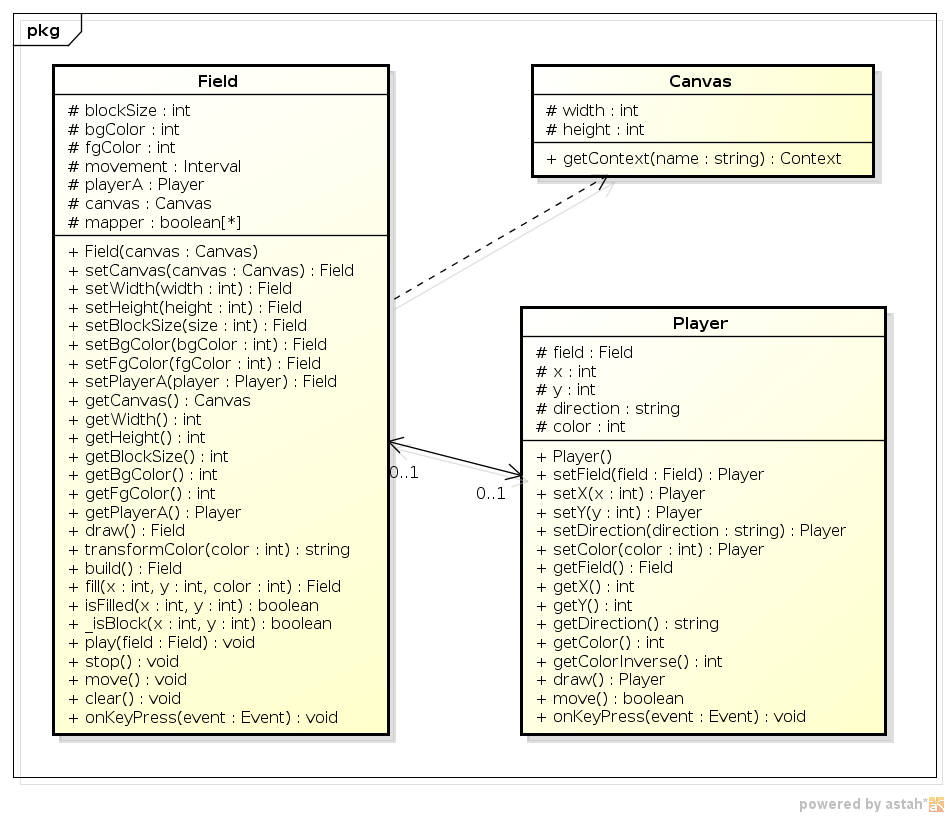
\includegraphics[scale=0.5]{class-diagram.png}
    \caption{Diagrama de Classes}
    \label{fig:diagram}
\end{figure}

O jogador é representado pela classe \texttt{jstron.player} e possui uma
referência ao campo de movimentação. O deslocamento do jogador é centralizado
nesta classe, solicitando ao campo permissão para avançar ao próximo bloco. Caso
este esteja ocupado, o bloco é renderizado em cor inversa a atual e o turno é
finalizado pelo campo. A movimentação do jogador é constante e pode ser alterada
utilizando as teclas específicas.

% Configuração Inicial ---------------------------------------------------------
\subsection{Configuração Inicial}

Objetos são inicializados no método \texttt{setup} da classe
\texttt{MainAssistant}. Estes são representantes do campo e jogador e recebem
configurações de cores e referências. Após, o campo é anexado à janela para
manter um acesso único a chamadas de retorno \emph{callbacks}. O campo
inicializa um temporizador para movimentar os jogadores e verificar as possíveis
colisões a cada 0,25 segundo.

Utilizando o \emph{framework} Mojo que pertence ao WebOS, foi incluído um botão
para que o usuário consiga reinicializar o campo quando pressionado. Para que a
cena que contém o campo seja apresentada, foi adicionado um empilhamento da cena
\texttt{main} no método \texttt{setup} da classe \texttt{StageAssistant}.

Na camada de visualização foi adicionado um elemento do tipo \texttt{canvas} que
é capturado para renderização do campo de movimento. Foram incluídos objetos que
são trabalhados pelo Mojo para estilizar o aplicativo conforme o WebOS. Também
foi utilizado folhas de estilo em cascata para formatar o aplicativo.

\begin{figure}
    \centering{}
    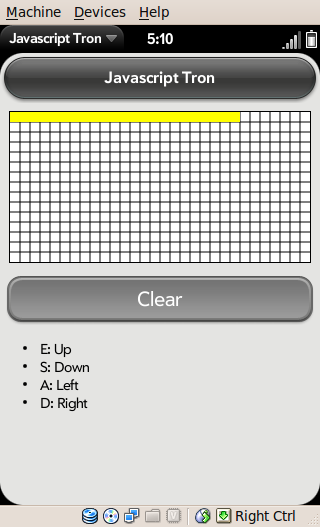
\includegraphics[scale=0.5]{screenshot.png}
    \caption{Máquina Virtual executando o Aplicativo}
    \label{fig:screenshot}
\end{figure}

O resultado final do aplicativo é apresentado na Figura \ref{fig:screenshot},
que exibe a execução do mesmo sobre a máquina virtual.

% Considerações Finais ---------------------------------------------------------
\section{Considerações Finais}
\label{sec:consideracoes}

Após assistir aos vídeos solicitados pela tarefa, entendi que um aplicativo em
WebOS é divido em duas estruturas básicas: estágios e cenas. Cada estágio é
representado por um cartão no aplicativo e as cenas são os conteúdos destes
cartões. A teoria de cartões existe para tornar a manipulação dos programas de
uma forma mais simples e intuitiva, modificando totalmente a teoria de janelas e
área de trabalho utilizada nos Sistemas Operacionais.

A documentação para desenvolvimento não é organizada e algumas vezes tornou a
leitura um pouco exaustiva com informações em múltiplas páginas. Também existem
ligações inválidas entre elas e a conexão segura HTTPS não é reconhecida como
confiável pelos navegadores.

O aplicativo desenvolvido possui somente um jogador e não deve ser considerado
como um aplicativo completo. Outro jogador poderá ser implementado porque a
estrutura foi desenvolvida com métodos isolados. Seria interessante a
comunicação via Bluetooth para jogos em dupla.

O WebOS tem uma \emph{interface} melhor trabalhada e intuitiva se comparada com
Android. A teoria de cartões fornece uma outra forma de trabalho sobre
aplicativos, algo que considerei muito interessante e atrativo. Por outro lado,
acho que o desenvolvimento sobre a plataforma ainda precisa crescer muito.

A questão de que aplicativos desenvolvidos em navegadores podem ser executados
com a mesma estrutura de classes no WebOS faz com que o dispositivo esteja cada
vez mais conectado a Internet, base de sua filosofia.

\end{document}
